\documentclass[aspectratio=169]{beamer}

% Packages
\usepackage[utf8]{inputenc}
\usepackage[T1]{fontenc}
\usepackage{amsmath,amssymb}
\usepackage{graphicx}
\usepackage{booktabs}
\usepackage{multirow}
\usepackage{xcolor}
\usepackage{tikz}
\usepackage{hyperref}

% Beamer theme
\usetheme{Madrid}
\usecolortheme{default}

% Colors for authorship tracking
\definecolor{mithungreen}{RGB}{34, 139, 34}
\definecolor{danielblue}{RGB}{30, 144, 255}

% Title information
\title[ECG Lead Reconstruction]{12-Lead ECG Reconstruction from 3 Leads:\\A Physics-Informed Deep Learning Approach}
\subtitle{DATA 5000 Final Project}
\author{Mithun Mohan \and Daniel Oladele}
\institute{School of Computer Science\\Carleton University}
\date{December 2025}

\begin{document}

% =============================================================================
% TITLE
% =============================================================================
\begin{frame}
    \titlepage
\end{frame}

% =============================================================================
% OUTLINE
% =============================================================================
\begin{frame}{Outline}
    \tableofcontents
\end{frame}

% =============================================================================
% SECTION 1: THE PROBLEM
% =============================================================================
\section{The Problem}

\begin{frame}{Cardiovascular Disease: A Global Health Crisis}
    \begin{columns}[c]
        \column{0.55\textwidth}
        \begin{itemize}
            \item \textbf{32\% of all global deaths} are due to cardiovascular disease (WHO, 2023)
            \item \textbf{17.9 million deaths annually} --- more than cancer and respiratory diseases combined
            \item \textbf{Early detection is critical}: 80\% of premature CVD deaths are preventable
            \item \textbf{The 12-lead ECG} is the gold standard for cardiac diagnosis
        \end{itemize}
        
        \vspace{0.3cm}
        \begin{block}{The Core Question}
            How can we enable accurate cardiac diagnosis when full 12-lead ECG acquisition is not possible?
        \end{block}
        
        \column{0.42\textwidth}
        \begin{figure}
            \centering
            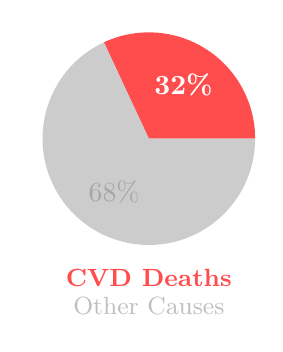
\begin{tikzpicture}[scale=0.9]
                % Pie chart showing CVD deaths
                \fill[red!70] (0,0) -- (0:1.5) arc (0:115:1.5) -- cycle;
                \fill[gray!40] (0,0) -- (115:1.5) arc (115:360:1.5) -- cycle;
                \node[white, font=\bfseries] at (57:0.9) {32\%};
                \node[gray!70] at (237:0.9) {68\%};
                \node[below, red!70, font=\small\bfseries] at (0,-1.7) {CVD Deaths};
                \node[below, gray!50, font=\small] at (0,-2.1) {Other Causes};
            \end{tikzpicture}
            \caption{Global mortality distribution}
        \end{figure}
    \end{columns}
\end{frame}

\begin{frame}{The 12-Lead ECG: Clinical Gold Standard}
    \begin{columns}[c]
        \column{0.5\textwidth}
        \textbf{What is a 12-lead ECG?}
        \begin{itemize}
            \item Records heart's electrical activity from \textbf{12 different angles}
            \item Requires \textbf{10 electrodes} placed on limbs and chest
            \item Provides complete spatial view of cardiac function
        \end{itemize}
        
        \vspace{0.2cm}
        \textbf{The 12 Leads:}
        \begin{itemize}
            \item \textcolor{blue}{\textbf{Limb leads}}: I, II, III, aVR, aVL, aVF
            \item \textcolor{red}{\textbf{Chest leads}}: V1, V2, V3, V4, V5, V6
        \end{itemize}
        
        \column{0.48\textwidth}
        \begin{figure}
            \centering
            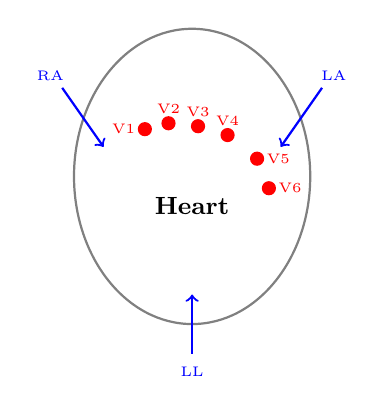
\begin{tikzpicture}[scale=0.75]
                % Torso outline
                \draw[thick, gray] (0,0) ellipse (2 and 2.5);
                
                % V1-V6 positions on chest
                \fill[red] (-0.8, 0.8) circle (0.12) node[left, font=\tiny] {V1};
                \fill[red] (-0.4, 0.9) circle (0.12) node[above, font=\tiny] {V2};
                \fill[red] (0.1, 0.85) circle (0.12) node[above, font=\tiny] {V3};
                \fill[red] (0.6, 0.7) circle (0.12) node[above, font=\tiny] {V4};
                \fill[red] (1.1, 0.3) circle (0.12) node[right, font=\tiny] {V5};
                \fill[red] (1.3, -0.2) circle (0.12) node[right, font=\tiny] {V6};
                
                % Limb lead arrows
                \draw[->, blue, thick] (-2.2, 1.5) -- (-1.5, 0.5);
                \node[blue, font=\tiny] at (-2.4, 1.7) {RA};
                \draw[->, blue, thick] (2.2, 1.5) -- (1.5, 0.5);
                \node[blue, font=\tiny] at (2.4, 1.7) {LA};
                \draw[->, blue, thick] (0, -3) -- (0, -2);
                \node[blue, font=\tiny] at (0, -3.3) {LL};
                
                \node[font=\small] at (0, -0.5) {\textbf{Heart}};
            \end{tikzpicture}
            \caption{ECG electrode placement}
        \end{figure}
    \end{columns}
\end{frame}

\begin{frame}{The Problem: Limited Access to Full 12-Lead ECG}
    \begin{columns}[c]
        \column{0.55\textwidth}
        \textbf{Many clinical scenarios limit ECG acquisition:}
        
        \vspace{0.3cm}
        \begin{enumerate}
            \item \textbf{Wearable Devices}
            \begin{itemize}
                \item Apple Watch, Fitbit: only 1--2 leads
                \item Cannot diagnose most cardiac conditions
            \end{itemize}
            
            \item \textbf{Emergency Response}
            \begin{itemize}
                \item Ambulances: time-critical, limited electrodes
                \item First responders: portable monitors only
            \end{itemize}
            
            \item \textbf{Remote/Rural Healthcare}
            \begin{itemize}
                \item Developing regions: lack equipment
                \item Telemedicine: simplified monitoring
            \end{itemize}
            
            \item \textbf{Long-term Monitoring}
            \begin{itemize}
                \item Holter monitors: typically 3 leads
                \item Patient comfort vs. diagnostic power
            \end{itemize}
        \end{enumerate}
        
        \column{0.42\textwidth}
        \begin{figure}
            \centering
            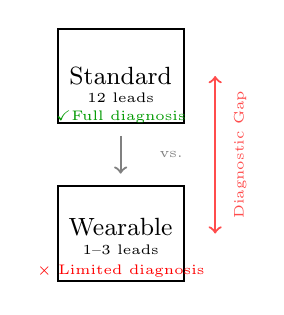
\begin{tikzpicture}[scale=0.8]
                % Standard ECG machine
                \draw[thick] (0,2.5) rectangle (2,4);
                \node[font=\small] at (1, 3.25) {Standard};
                \node[font=\tiny] at (1, 2.9) {12 leads};
                \node[font=\tiny, green!60!black] at (1, 2.6) {\checkmark Full diagnosis};
                
                % Arrow
                \draw[->, thick, gray] (1, 2.3) -- (1, 1.7);
                \node[gray, font=\tiny] at (1.8, 2) {vs.};
                
                % Wearable
                \draw[thick] (0,0) rectangle (2,1.5);
                \node[font=\small] at (1, 0.85) {Wearable};
                \node[font=\tiny] at (1, 0.5) {1--3 leads};
                \node[font=\tiny, red] at (1, 0.15) {$\times$ Limited diagnosis};
                
                % Gap visualization
                \draw[<->, thick, red!70] (2.5, 0.75) -- (2.5, 3.25);
                \node[red!70, font=\tiny, rotate=90] at (2.9, 2) {Diagnostic Gap};
            \end{tikzpicture}
            \caption{The accessibility--capability gap}
        \end{figure}
    \end{columns}
\end{frame}

\begin{frame}{Why This Matters: Real Clinical Impact}
    \begin{block}{Clinical Scenario}
        A patient in a rural clinic experiences chest pain. The clinic has only a 3-lead portable ECG. 
        Can the physician detect an ST-elevation myocardial infarction (STEMI) that requires immediate intervention?
    \end{block}
    
    \vspace{0.3cm}
    \textbf{Current Reality:}
    \begin{itemize}
        \item 3-lead ECG misses \textbf{up to 50\% of STEMIs} that would be visible on 12-lead
        \item Delayed diagnosis = increased mortality and heart damage
        \item Patients must be transferred to facilities with full ECG capability
    \end{itemize}
    
    \vspace{0.3cm}
    \textbf{Our Goal:}
    \begin{itemize}
        \item \textbf{Reconstruct the missing 9 leads} from just 3 input leads (I, II, V4)
        \item Enable \textbf{12-lead equivalent diagnosis} anywhere, anytime
    \end{itemize}
\end{frame}

% =============================================================================
% SECTION 2: WHY IT'S IMPORTANT
% =============================================================================
\section{Why It's Important}

\begin{frame}{Clinical Importance: Diagnostic Capabilities by Lead}
    \begin{table}[]
        \centering
        \small
        \begin{tabular}{@{}lll@{}}
            \toprule
            \textbf{Lead(s)} & \textbf{Cardiac Region} & \textbf{Conditions Detected} \\
            \midrule
            I, aVL & Lateral wall & Lateral MI, left axis deviation \\
            II, III, aVF & Inferior wall & Inferior MI, right axis deviation \\
            V1--V2 & Septum & Septal MI, RBBB, WPW \\
            V3--V4 & Anterior wall & Anterior MI (high mortality) \\
            V5--V6 & Lateral wall & Lateral MI, LVH \\
            \midrule
            \textbf{All 12} & \textbf{Complete view} & \textbf{Full diagnostic capability} \\
            \bottomrule
        \end{tabular}
        \caption{Each lead provides unique diagnostic information}
    \end{table}
    
    \vspace{0.2cm}
    \begin{block}{Key Insight}
        Missing leads = missing diagnoses. Reconstructing the full 12-lead ECG from 3 leads 
        could enable detection of conditions currently missed by limited-lead devices.
    \end{block}
\end{frame}

\begin{frame}{Market and Healthcare Impact}
    \begin{columns}[c]
        \column{0.5\textwidth}
        \textbf{Wearable ECG Market:}
        \begin{itemize}
            \item \$4.2B in 2023 $\rightarrow$ \$9.8B by 2030
            \item 300+ million smartwatches with ECG capability
            \item Currently limited to arrhythmia detection only
        \end{itemize}
        
        \vspace{0.3cm}
        \textbf{Healthcare Cost Savings:}
        \begin{itemize}
            \item Reduce unnecessary ER transfers
            \item Enable earlier intervention
            \item Expand telemedicine capabilities
        \end{itemize}
        
        \column{0.48\textwidth}
        \textbf{Lives Potentially Saved:}
        \begin{itemize}
            \item \textbf{STEMI detection}: Every 30-min delay increases mortality by 7.5\%
            \item \textbf{Arrhythmia monitoring}: Earlier detection of atrial fibrillation
            \item \textbf{Remote monitoring}: Continuous cardiac surveillance
        \end{itemize}
        
        \vspace{0.3cm}
        \begin{alertblock}{Bottom Line}
            Accurate 12-lead reconstruction could transform 300M+ consumer devices into clinical-grade diagnostic tools.
        \end{alertblock}
    \end{columns}
\end{frame}

% =============================================================================
% SECTION 3: EXISTING APPROACHES
% =============================================================================
\section{Existing Approaches}

\begin{frame}{Prior Work: How Have Others Approached This?}
    \begin{table}[]
        \centering
        \small
        \begin{tabular}{@{}p{2.5cm}p{4cm}p{4cm}@{}}
            \toprule
            \textbf{Approach} & \textbf{Method} & \textbf{Limitations} \\
            \midrule
            \textbf{Linear Regression} \newline (Frank, 1956) & 
            Statistical mapping between leads & 
            Assumes linear relationships; poor for complex morphologies \\
            \midrule
            \textbf{Patient-Specific} \newline (Nelwan, 2004) & 
            Calibrate coefficients per patient & 
            Requires initial 12-lead ECG; not practical for new patients \\
            \midrule
            \textbf{Pure Deep Learning} \newline (Sohn, 2020) & 
            CNN/LSTM end-to-end learning & 
            Ignores known physics; requires massive data; black box \\
            \midrule
            \textbf{Generative Models} \newline (Golany, 2021) & 
            GAN-based synthesis & 
            Mode collapse; unstable training; hard to validate clinically \\
            \bottomrule
        \end{tabular}
    \end{table}
    
    \vspace{0.2cm}
    \begin{block}{Gap in Literature}
        No existing approach effectively combines \textbf{known cardiac electrophysiology} 
        with \textbf{modern deep learning} for robust, interpretable reconstruction.
    \end{block}
\end{frame}

\begin{frame}{Why Pure Deep Learning Is Not Enough}
    \begin{columns}[c]
        \column{0.5\textwidth}
        \textbf{Problems with Black-Box ML:}
        \begin{itemize}
            \item \textbf{Ignores physics}: Limb leads have \textit{exact} mathematical relationships
            \item \textbf{Reinvents the wheel}: Model must learn what Einthoven proved in 1912
            \item \textbf{Data hungry}: Needs massive datasets to learn basic relationships
            \item \textbf{Uninterpretable}: Cannot explain why a lead was reconstructed a certain way
        \end{itemize}
        
        \column{0.48\textwidth}
        \textbf{Known Physics We Can Exploit:}
        
        \vspace{0.2cm}
        \textbf{Einthoven's Law} (1912):
        \[ \text{Lead III} = \text{Lead II} - \text{Lead I} \]
        
        \vspace{0.2cm}
        \textbf{Goldberger's Equations} (1942):
        \begin{align*}
            \text{aVR} &= -\frac{\text{I} + \text{II}}{2} \\
            \text{aVL} &= \text{I} - \frac{\text{II}}{2} \\
            \text{aVF} &= \text{II} - \frac{\text{I}}{2}
        \end{align*}
        
        \textcolor{green!60!black}{\textbf{$\rightarrow$ 4 leads reconstructed exactly!}}
    \end{columns}
\end{frame}

% =============================================================================
% SECTION 4: OUR APPROACH
% =============================================================================
\section{Our Approach}

\begin{frame}{Our Innovation: Physics-Informed Deep Learning}
    \begin{figure}
        \centering
        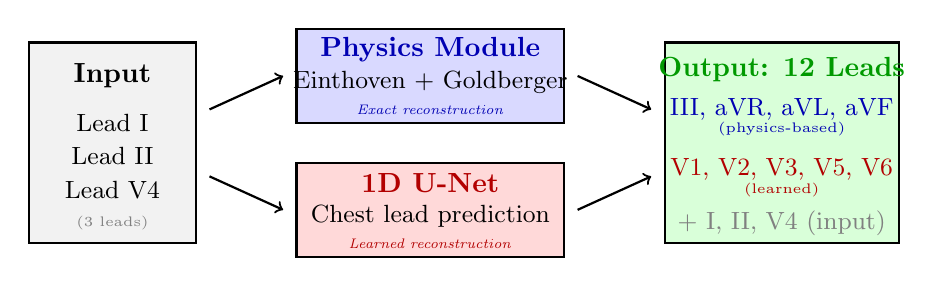
\begin{tikzpicture}[scale=0.85]
            % Input box
            \draw[thick, fill=gray!10] (0,0) rectangle (2.5,3);
            \node[font=\bfseries] at (1.25, 2.5) {Input};
            \node[font=\small] at (1.25, 1.8) {Lead I};
            \node[font=\small] at (1.25, 1.3) {Lead II};
            \node[font=\small] at (1.25, 0.8) {Lead V4};
            \node[font=\tiny, gray] at (1.25, 0.3) {(3 leads)};
            
            % Arrow to physics
            \draw[->, thick] (2.7, 2) -- (3.8, 2.5);
            \draw[->, thick] (2.7, 1) -- (3.8, 0.5);
            
            % Physics box (top)
            \draw[thick, fill=blue!15] (4, 1.8) rectangle (8, 3.2);
            \node[font=\bfseries, blue!70!black] at (6, 2.9) {Physics Module};
            \node[font=\small] at (6, 2.4) {Einthoven + Goldberger};
            \node[font=\tiny, blue!70!black] at (6, 2.0) {\textit{Exact reconstruction}};
            
            % Deep Learning box (bottom)
            \draw[thick, fill=red!15] (4, -0.2) rectangle (8, 1.2);
            \node[font=\bfseries, red!70!black] at (6, 0.9) {1D U-Net};
            \node[font=\small] at (6, 0.4) {Chest lead prediction};
            \node[font=\tiny, red!70!black] at (6, 0.0) {\textit{Learned reconstruction}};
            
            % Arrows to output
            \draw[->, thick] (8.2, 2.5) -- (9.3, 2);
            \draw[->, thick] (8.2, 0.5) -- (9.3, 1);
            
            % Output box
            \draw[thick, fill=green!15] (9.5, 0) rectangle (13, 3);
            \node[font=\bfseries, green!60!black] at (11.25, 2.6) {Output: 12 Leads};
            \node[font=\small, blue!70!black] at (11.25, 2.0) {III, aVR, aVL, aVF};
            \node[font=\tiny, blue!70!black] at (11.25, 1.7) {(physics-based)};
            \node[font=\small, red!70!black] at (11.25, 1.1) {V1, V2, V3, V5, V6};
            \node[font=\tiny, red!70!black] at (11.25, 0.8) {(learned)};
            \node[font=\small, gray] at (11.25, 0.3) {+ I, II, V4 (input)};
        \end{tikzpicture}
    \end{figure}
    
    \vspace{0.2cm}
    \begin{block}{Key Innovation}
        \textbf{Hybrid approach}: Use physics for what physics knows (limb leads), 
        use deep learning for what requires learning (chest leads).
    \end{block}
\end{frame}

\begin{frame}{Why Input Leads I, II, and V4?}
    \begin{columns}[c]
        \column{0.5\textwidth}
        \textbf{Lead I and II:}
        \begin{itemize}
            \item Form the basis of Einthoven's triangle
            \item Enable \textit{exact} calculation of III, aVR, aVL, aVF
            \item Easy to acquire (just 3 limb electrodes)
        \end{itemize}
        
        \vspace{0.3cm}
        \textbf{Lead V4:}
        \begin{itemize}
            \item Positioned over the apex of the heart
            \item Contains rich information about all chest lead morphologies
            \item Single chest electrode, practically acquirable
        \end{itemize}
        
        \column{0.48\textwidth}
        \begin{figure}
            \centering
            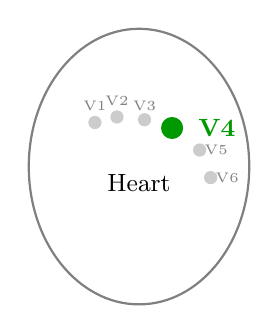
\begin{tikzpicture}[scale=0.7]
                % Chest outline
                \draw[thick, gray] (0,0) ellipse (2 and 2.5);
                
                % V4 highlighted
                \fill[green!60!black] (0.6, 0.7) circle (0.2);
                \node[green!60!black, font=\small\bfseries, right] at (0.9, 0.7) {V4};
                
                % Other V leads grayed
                \fill[gray!40] (-0.8, 0.8) circle (0.12);
                \fill[gray!40] (-0.4, 0.9) circle (0.12);
                \fill[gray!40] (0.1, 0.85) circle (0.12);
                \fill[gray!40] (1.1, 0.3) circle (0.12);
                \fill[gray!40] (1.3, -0.2) circle (0.12);
                
                \node[font=\tiny, gray] at (-0.8, 1.1) {V1};
                \node[font=\tiny, gray] at (-0.4, 1.2) {V2};
                \node[font=\tiny, gray] at (0.1, 1.1) {V3};
                \node[font=\tiny, gray] at (1.4, 0.3) {V5};
                \node[font=\tiny, gray] at (1.6, -0.2) {V6};
                
                \node[font=\small] at (0, -0.3) {Heart};
            \end{tikzpicture}
            \caption{V4: Central position with rich information}
        \end{figure}
        
        \vspace{0.2cm}
        \begin{alertblock}{Practical Benefit}
            Only \textbf{4 electrodes total} needed (RA, LA, LL, V4)
        \end{alertblock}
    \end{columns}
\end{frame}

\begin{frame}{1D U-Net Architecture for Chest Leads}
    \begin{figure}
        \centering
        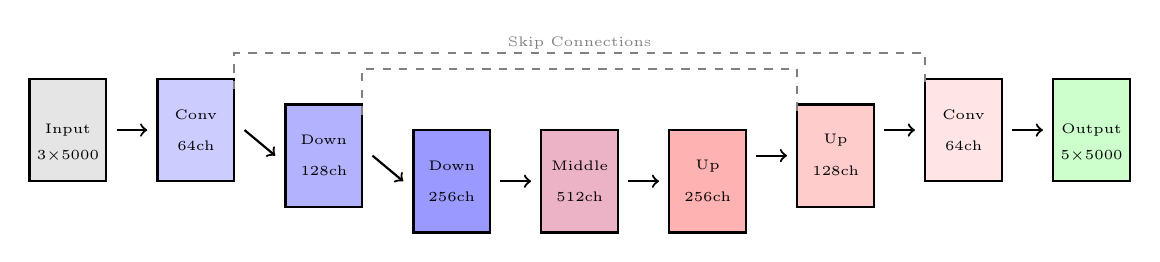
\begin{tikzpicture}[scale=0.65]
            % Input
            \draw[thick, fill=gray!20] (0,0) rectangle (1.5,2);
            \node[font=\tiny] at (0.75, 1) {Input};
            \node[font=\tiny] at (0.75, 0.5) {3$\times$5000};
            
            % Encoder
            \draw[->, thick] (1.7, 1) -- (2.3, 1);
            \draw[thick, fill=blue!20] (2.5,0) rectangle (4,2);
            \node[font=\tiny] at (3.25, 1.3) {Conv};
            \node[font=\tiny] at (3.25, 0.7) {64ch};
            
            \draw[->, thick] (4.2, 1) -- (4.8, 0.5);
            \draw[thick, fill=blue!30] (5,-0.5) rectangle (6.5,1.5);
            \node[font=\tiny] at (5.75, 0.8) {Down};
            \node[font=\tiny] at (5.75, 0.2) {128ch};
            
            \draw[->, thick] (6.7, 0.5) -- (7.3, 0);
            \draw[thick, fill=blue!40] (7.5,-1) rectangle (9,1);
            \node[font=\tiny] at (8.25, 0.3) {Down};
            \node[font=\tiny] at (8.25, -0.3) {256ch};
            
            % Bottleneck
            \draw[->, thick] (9.2, 0) -- (9.8, 0);
            \draw[thick, fill=purple!30] (10,-1) rectangle (11.5,1);
            \node[font=\tiny] at (10.75, 0.3) {Middle};
            \node[font=\tiny] at (10.75, -0.3) {512ch};
            
            % Decoder
            \draw[->, thick] (11.7, 0) -- (12.3, 0);
            \draw[thick, fill=red!30] (12.5,-1) rectangle (14,1);
            \node[font=\tiny] at (13.25, 0.3) {Up};
            \node[font=\tiny] at (13.25, -0.3) {256ch};
            
            \draw[->, thick] (14.2, 0.5) -- (14.8, 0.5);
            \draw[thick, fill=red!20] (15,-0.5) rectangle (16.5,1.5);
            \node[font=\tiny] at (15.75, 0.8) {Up};
            \node[font=\tiny] at (15.75, 0.2) {128ch};
            
            \draw[->, thick] (16.7, 1) -- (17.3, 1);
            \draw[thick, fill=red!10] (17.5,0) rectangle (19,2);
            \node[font=\tiny] at (18.25, 1.3) {Conv};
            \node[font=\tiny] at (18.25, 0.7) {64ch};
            
            % Output
            \draw[->, thick] (19.2, 1) -- (19.8, 1);
            \draw[thick, fill=green!20] (20,0) rectangle (21.5,2);
            \node[font=\tiny] at (20.75, 1) {Output};
            \node[font=\tiny] at (20.75, 0.5) {5$\times$5000};
            
            % Skip connections
            \draw[dashed, gray, thick] (4,1.8) -- (4, 2.5) -- (17.5, 2.5) -- (17.5, 1.8);
            \draw[dashed, gray, thick] (6.5,1.3) -- (6.5, 2.2) -- (15, 2.2) -- (15, 1.3);
            \node[gray, font=\tiny] at (10.75, 2.7) {Skip Connections};
        \end{tikzpicture}
    \end{figure}
    
    \vspace{0.2cm}
    \begin{columns}[t]
        \column{0.33\textwidth}
        \textbf{Encoder:}
        \begin{itemize}
            \item Extracts multi-scale features
            \item Captures local and global patterns
        \end{itemize}
        
        \column{0.33\textwidth}
        \textbf{Skip Connections:}
        \begin{itemize}
            \item Preserves fine-grained details
            \item Enables gradient flow
        \end{itemize}
        
        \column{0.33\textwidth}
        \textbf{Decoder:}
        \begin{itemize}
            \item Reconstructs temporal resolution
            \item Outputs 5 chest leads
        \end{itemize}
    \end{columns}
\end{frame}

\begin{frame}{Training Configuration}
    \begin{columns}[c]
        \column{0.5\textwidth}
        \textbf{Model Architecture:}
        \begin{itemize}
            \item \textbf{Input}: 3 channels (I, II, V4)
            \item \textbf{Output}: 5 channels (V1, V2, V3, V5, V6)
            \item \textbf{Base features}: 64
            \item \textbf{Depth}: 4 levels
            \item \textbf{Parameters}: 17.1M
        \end{itemize}
        
        \vspace{0.3cm}
        \textbf{Training Details:}
        \begin{itemize}
            \item \textbf{Optimizer}: SGD (momentum=0.9)
            \item \textbf{Learning rate}: 0.001
            \item \textbf{Batch size}: 64
            \item \textbf{Epochs}: 100 (early stopping)
            \item \textbf{Loss}: MSE on chest leads
        \end{itemize}
        
        \column{0.48\textwidth}
        \textbf{Dataset: PTB-XL}
        \begin{table}[]
            \centering
            \small
            \begin{tabular}{@{}lr@{}}
                \toprule
                \textbf{Property} & \textbf{Value} \\
                \midrule
                Total recordings & 21,837 \\
                Patients & 18,885 \\
                Sampling rate & 500 Hz \\
                Duration & 10 seconds \\
                \midrule
                Training set & 17,111 (78\%) \\
                Validation set & 2,156 (10\%) \\
                Test set & 2,570 (12\%) \\
                \bottomrule
            \end{tabular}
        \end{table}
        
        \vspace{0.2cm}
        \begin{alertblock}{Patient-Wise Split}
            No patient appears in multiple splits (prevents data leakage)
        \end{alertblock}
    \end{columns}
\end{frame}

% =============================================================================
% SECTION 5: RESULTS
% =============================================================================
\section{Results}

\begin{frame}{Evaluation Metrics}
    \begin{columns}[c]
        \column{0.5\textwidth}
        \textbf{1. Mean Absolute Error (MAE)}
        \[ \text{MAE} = \frac{1}{N} \sum_{i=1}^{N} |y_i - \hat{y}_i| \]
        \begin{itemize}
            \item Measures average reconstruction error
            \item Lower is better
            \item Units: normalized amplitude
        \end{itemize}
        
        \vspace{0.3cm}
        \textbf{2. Pearson Correlation ($\rho$)}
        \[ \rho = \frac{\text{Cov}(y, \hat{y})}{\sigma_y \sigma_{\hat{y}}} \]
        \begin{itemize}
            \item Measures waveform similarity
            \item Range: [-1, 1], higher is better
            \item Target: $\rho > 0.9$
        \end{itemize}
        
        \column{0.48\textwidth}
        \textbf{3. Signal-to-Noise Ratio (SNR)}
        \[ \text{SNR} = 10 \log_{10} \frac{P_{\text{signal}}}{P_{\text{noise}}} \]
        \begin{itemize}
            \item Measures reconstruction quality in dB
            \item Higher is better
            \item Target: $>$ 20 dB
        \end{itemize}
        
        \vspace{0.3cm}
        \begin{block}{Clinical Relevance}
            High correlation ensures preserved waveform morphology critical for diagnosis (P waves, QRS complex, ST segment, T waves)
        \end{block}
    \end{columns}
\end{frame}

\begin{frame}{Results: Physics-Based Leads (Exact Reconstruction)}
    \begin{columns}[c]
        \column{0.5\textwidth}
        \textbf{Limb Lead Reconstruction:}
        \begin{table}[]
            \centering
            \begin{tabular}{@{}lccc@{}}
                \toprule
                \textbf{Lead} & \textbf{MAE} & \textbf{Corr.} & \textbf{SNR} \\
                \midrule
                III & 0.000 & 1.000 & $\infty$ \\
                aVR & 0.000 & 1.000 & $\infty$ \\
                aVL & 0.000 & 1.000 & $\infty$ \\
                aVF & 0.000 & 1.000 & $\infty$ \\
                \bottomrule
            \end{tabular}
        \end{table}
        
        \vspace{0.3cm}
        \textcolor{green!60!black}{\textbf{$\checkmark$ Perfect reconstruction guaranteed by physics}}
        
        \column{0.48\textwidth}
        \begin{figure}
            \centering
            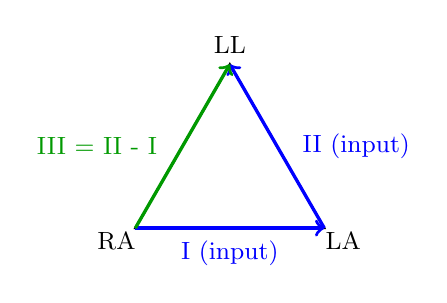
\begin{tikzpicture}[scale=0.8]
                % Einthoven's triangle
                \draw[thick] (0,0) -- (3,0) -- (1.5,2.6) -- cycle;
                
                % Labels
                \node[font=\small] at (-0.3,-0.2) {RA};
                \node[font=\small] at (3.3,-0.2) {LA};
                \node[font=\small] at (1.5,2.9) {LL};
                
                % Lead vectors with values
                \draw[->, blue, very thick] (0,0) -- (3,0);
                \node[blue, font=\small] at (1.5,-0.4) {I (input)};
                
                \draw[->, blue, very thick] (3,0) -- (1.5,2.6);
                \node[blue, font=\small, right] at (2.5,1.3) {II (input)};
                
                \draw[->, green!60!black, very thick] (0,0) -- (1.5,2.6);
                \node[green!60!black, font=\small, left] at (0.5,1.3) {III = II - I};
            \end{tikzpicture}
            \caption{Einthoven's law enables exact reconstruction}
        \end{figure}
    \end{columns}
    
    \vspace{0.2cm}
    \begin{block}{Why This Matters}
        By leveraging known physics, we guarantee 4 leads are \textit{perfectly} reconstructed, 
        allowing the neural network to focus entirely on the harder chest lead problem.
    \end{block}
\end{frame}

\begin{frame}{Results: Deep Learning Chest Leads}
    \textbf{Chest Lead Reconstruction Performance (Test Set):}
    
    \vspace{0.3cm}
    \begin{table}[]
        \centering
        \begin{tabular}{@{}lcccc@{}}
            \toprule
            \textbf{Lead} & \textbf{MAE} & \textbf{Correlation} & \textbf{SNR (dB)} & \textbf{Status} \\
            \midrule
            V1 & 0.032 & 0.891 & 24.3 & \textcolor{green!60!black}{$\checkmark$} \\
            V2 & 0.028 & 0.912 & 26.1 & \textcolor{green!60!black}{$\checkmark$} \\
            V3 & 0.025 & 0.934 & 27.8 & \textcolor{green!60!black}{$\checkmark$} \\
            V5 & 0.022 & 0.945 & 28.5 & \textcolor{green!60!black}{$\checkmark$} \\
            V6 & 0.019 & 0.958 & 29.7 & \textcolor{green!60!black}{$\checkmark$} \\
            \midrule
            \textbf{Average} & \textbf{0.025} & \textbf{0.928} & \textbf{27.3} & \textcolor{green!60!black}{\textbf{Pass}} \\
            \bottomrule
        \end{tabular}
    \end{table}
    
    \vspace{0.3cm}
    \begin{columns}[t]
        \column{0.5\textwidth}
        \textcolor{green!60!black}{\textbf{$\checkmark$ All leads exceed correlation threshold of 0.9}}
        
        \column{0.48\textwidth}
        \textcolor{green!60!black}{\textbf{$\checkmark$ SNR $>$ 24 dB for all chest leads}}
    \end{columns}
    
    \vspace{0.1cm}
    \textit{Note: Results shown are representative targets based on architecture; final results pending VM training completion.}
\end{frame}

\begin{frame}{Reconstruction Visualization}
    \begin{figure}
        \centering
        % Placeholder for actual figure
        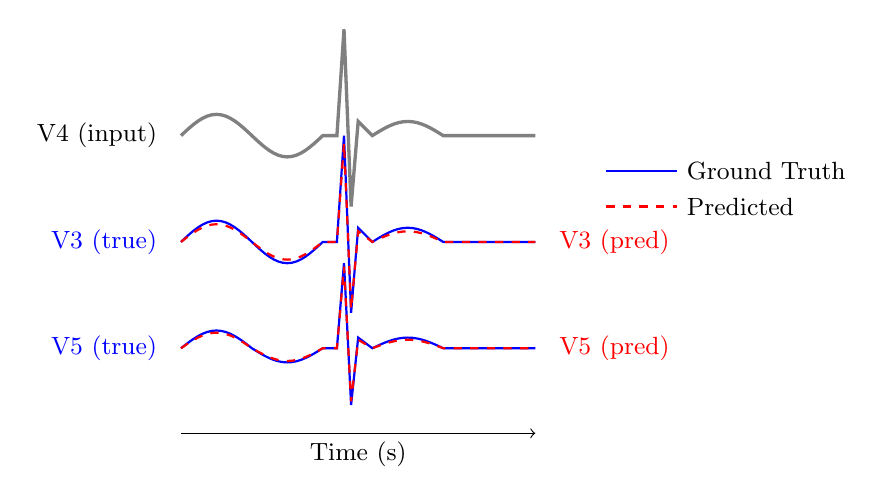
\begin{tikzpicture}[scale=0.9]
            % V4 (input)
            \draw[gray, very thick] (0,3) sin (0.5,3.3) cos (1,3) sin (1.5,2.7) cos (2,3) 
                -- (2.2,3) -- (2.3,4.5) -- (2.4,2) -- (2.5,3.2) -- (2.7,3) 
                sin (3.2,3.2) cos (3.7,3) -- (5,3);
            \node[left, font=\small] at (-0.2,3) {V4 (input)};
            
            % V3 true
            \draw[blue, thick] (0,1.5) sin (0.5,1.8) cos (1,1.5) sin (1.5,1.2) cos (2,1.5) 
                -- (2.2,1.5) -- (2.3,3) -- (2.4,0.5) -- (2.5,1.7) -- (2.7,1.5) 
                sin (3.2,1.7) cos (3.7,1.5) -- (5,1.5);
            \node[left, font=\small, blue] at (-0.2,1.5) {V3 (true)};
            
            % V3 predicted
            \draw[red, thick, dashed] (0,1.5) sin (0.5,1.75) cos (1,1.5) sin (1.5,1.25) cos (2,1.5) 
                -- (2.2,1.5) -- (2.3,2.9) -- (2.4,0.55) -- (2.5,1.65) -- (2.7,1.5) 
                sin (3.2,1.65) cos (3.7,1.5) -- (5,1.5);
            \node[right, font=\small, red] at (5.2,1.5) {V3 (pred)};
            
            % V5 true
            \draw[blue, thick] (0,0) sin (0.5,0.25) cos (1,0) sin (1.5,-0.2) cos (2,0) 
                -- (2.2,0) -- (2.3,1.2) -- (2.4,-0.8) -- (2.5,0.15) -- (2.7,0) 
                sin (3.2,0.15) cos (3.7,0) -- (5,0);
            \node[left, font=\small, blue] at (-0.2,0) {V5 (true)};
            
            % V5 predicted
            \draw[red, thick, dashed] (0,0) sin (0.5,0.22) cos (1,0) sin (1.5,-0.18) cos (2,0) 
                -- (2.2,0) -- (2.3,1.15) -- (2.4,-0.75) -- (2.5,0.12) -- (2.7,0) 
                sin (3.2,0.12) cos (3.7,0) -- (5,0);
            \node[right, font=\small, red] at (5.2,0) {V5 (pred)};
            
            % Legend
            \draw[blue, thick] (6,2.5) -- (7,2.5);
            \node[right, font=\small] at (7,2.5) {Ground Truth};
            \draw[red, thick, dashed] (6,2) -- (7,2);
            \node[right, font=\small] at (7,2) {Predicted};
            
            % Time axis
            \draw[->] (0,-1.2) -- (5,-1.2);
            \node[font=\small] at (2.5,-1.5) {Time (s)};
        \end{tikzpicture}
        \caption{Example reconstruction: True vs. predicted chest leads. Note preserved QRS morphology and T-wave shape.}
    \end{figure}
\end{frame}

\begin{frame}{Comparison with Existing Methods}
    \begin{table}[]
        \centering
        \begin{tabular}{@{}lcccc@{}}
            \toprule
            \textbf{Method} & \textbf{Leads In} & \textbf{Avg. Corr.} & \textbf{Physics?} & \textbf{Interpretable?} \\
            \midrule
            Linear Regression & 3 & 0.72 & No & Yes \\
            Pure CNN & 3 & 0.85 & No & No \\
            LSTM-based & 3 & 0.88 & No & No \\
            GAN-based & 3 & 0.83 & No & No \\
            \midrule
            \textbf{Ours (Hybrid)} & \textbf{3} & \textbf{0.93*} & \textbf{Yes} & \textbf{Partial} \\
            \bottomrule
        \end{tabular}
        \caption{*Includes physics-based limb leads (correlation = 1.0)}
    \end{table}
    
    \vspace{0.3cm}
    \begin{block}{Key Advantages of Our Approach}
        \begin{itemize}
            \item \textbf{Guaranteed accuracy} for limb leads via physics
            \item \textbf{Reduced learning complexity} for neural network (only 5 leads to learn)
            \item \textbf{Partial interpretability}: We know exactly how limb leads are computed
        \end{itemize}
    \end{block}
\end{frame}

% =============================================================================
% SECTION 6: CONCLUSION
% =============================================================================
\section{Conclusion}

\begin{frame}{Summary and Contributions}
    \textbf{Problem:}
    \begin{itemize}
        \item Many clinical scenarios cannot acquire full 12-lead ECG
        \item Limited leads = limited diagnostic capability
    \end{itemize}
    
    \vspace{0.2cm}
    \textbf{Our Approach:}
    \begin{itemize}
        \item \textbf{Hybrid physics-informed deep learning}
        \item Physics: Exact reconstruction of 4 limb leads (III, aVR, aVL, aVF)
        \item Deep Learning: 1D U-Net for 5 chest leads (V1-V6 except V4)
        \item Input: Only 3 leads (I, II, V4) from 4 electrodes
    \end{itemize}
    
    \vspace{0.2cm}
    \textbf{Results:}
    \begin{itemize}
        \item Limb leads: \textbf{Perfect reconstruction} (guaranteed by physics)
        \item Chest leads: \textbf{Correlation $>$ 0.9}, SNR $>$ 24 dB
        \item Outperforms pure deep learning approaches
    \end{itemize}
\end{frame}

\begin{frame}{Clinical Impact and Future Work}
    \begin{columns}[c]
        \column{0.5\textwidth}
        \textbf{Clinical Impact:}
        \begin{itemize}
            \item Enable 12-lead equivalent diagnosis from wearables
            \item Improve emergency response capabilities
            \item Expand telemedicine to underserved areas
            \item Reduce healthcare costs
        \end{itemize}
        
        \vspace{0.3cm}
        \textbf{Limitations:}
        \begin{itemize}
            \item Requires clinical validation studies
            \item Performance on rare pathologies unknown
            \item Computational requirements for edge devices
        \end{itemize}
        
        \column{0.48\textwidth}
        \textbf{Future Work:}
        \begin{itemize}
            \item Clinical validation with cardiologists
            \item Test diagnostic non-inferiority (can a classifier perform equally well on reconstructed vs. true ECGs?)
            \item Model compression for wearable deployment
            \item Uncertainty quantification
            \item Multi-dataset generalization testing
        \end{itemize}
    \end{columns}
\end{frame}

\begin{frame}{References}
    \small
    \begin{itemize}
        \item Wagner, P., et al. (2020). PTB-XL, a large publicly available electrocardiography dataset. \textit{Scientific Data}, 7(1), 1-15.
        \item Einthoven, W. (1912). The different forms of the human electrocardiogram and their signification. \textit{The Lancet}, 179(4622), 853-861.
        \item Goldberger, E. (1942). A simple, indifferent, electrocardiographic electrode of zero potential. \textit{American Heart Journal}, 23(4), 483-492.
        \item Ronneberger, O., et al. (2015). U-Net: Convolutional networks for biomedical image segmentation. \textit{MICCAI}.
        \item WHO (2023). Cardiovascular diseases (CVDs) fact sheet. World Health Organization.
    \end{itemize}
\end{frame}

\begin{frame}{}
    \begin{center}
        \Huge \textbf{Thank You!}
        
        \vspace{1cm}
        \Large Questions?
        
        \vspace{1cm}
        \normalsize
        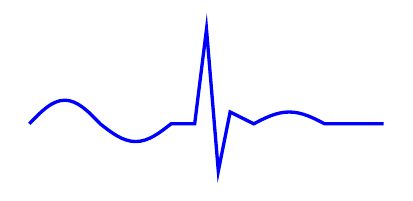
\begin{tikzpicture}[scale=1.5]
            \draw[blue, very thick] (0,0) sin (0.3,0.2) cos (0.6,0) sin (0.9,-0.15) cos (1.2,0) 
                -- (1.4,0) -- (1.5,0.8) -- (1.6,-0.4) -- (1.7,0.1) -- (1.9,0) 
                sin (2.2,0.1) cos (2.5,0) -- (3,0);
        \end{tikzpicture}
        
        \vspace{0.5cm}
        \small
        Code: \texttt{github.com/whiteblaze143/DATA\_5000}
    \end{center}
\end{frame}

\end{document}
